\documentclass{article}
\usepackage{graphicx}
\usepackage{fancyhdr}
\usepackage{listings}

\let\<\textless
\let\>\textgreater

\graphicspath{ {images/} }
\pagestyle{fancy}
\fancyhf{}
\rhead{Proyecto \#2}
\rfoot{P\'agina \thepage}

\begin{document}
\begin{titlepage}
  \centering
  {\scshape\LARGE Instituto Tecnol\'ogico de Costa Rica \par}
  \vspace{1cm}
  {\scshape\Large Proyecto \#2\par}
  \vspace{1.5cm}
  {\Large\itshape Alejandro Rojas\par}
  {\Large\itshape Sa\'ul Zamora\par}
  \vfill
  profesor\par
  Kevin Moraga \textsc{}

  \vfill

% Bottom of the page
  {\large \today\par}
\end{titlepage}

\section{Introducci\'on}
Se requiere un sistema para una empresa productora de dispositivos de IoT (Internet Of Things), los cuales se distribuyen a nivel nacional y se exporta a Nicaragua, Panam\'a y Guatemala.

Uno de los principales negocios de la empresa son las ``Smart Houses'', lo cual implica brindarle al cliente una experiencia \'unica al darle control total de su casa y los dispositivos en ella.

Las bases de datos deben almacenar informaci\'on de forma local y otros datos de forma remota en las instalaciones de la empresa. Actualmente, las tecnolog\'ias usadas son MySQL, SQL Server y Oracle.

La base de datos de producci\'on posee un inventario de todas las partes que la empresa adquiere como materia prima para la creaci\'on de los dispositivos. Existe otro sistema que usa otra base de datos donde se controlan las ventas de los productos y dispositivos, la cual es b\'asicamente un cat\'alogo de los productos; adem\'as de un historial con los cambios en los precios de dichos productos.

Cada casa de habitaci\'on cuenta con una base de datos local, cuya funci\'on principal es recolectar informaci\'on post-venta de los dispositivos e informaci\'on generada por su uso.

Es requerido mantener las bases de datos locales y remotas replicadas para brindarle al usuario la experiencia que desea.

Adem\'as, el sistema deseado debe ser capaz de producir estad\'isticas sobre inteligencia de negocios con el fin de ayudar a la gerencia a tomar decisiones m\'as acertadas. Algunos de los puntos m\'as relevantes son:

\begin{itemize}
  \item Costos de producci\'on
  \item Sugerencias de consumo de productos del cliente en los pr\'oximos 15 d\'ias.
  \item Dispositivos IoT m\'as utilizados por un cliente
  \item Dispositivos IoT m\'as vendidos
  \item Tiempo de entrega de materiales relacionados a los dispositivos IoT m\'as vendidos
  \item Estad\'isticas sobre los proveedores (tiempos de respuesta, calidad de materiales, etc)
  \item Determinar los materiales de mayor y menor circulaci\'on
  \item Estad\'isticas sobre las ventas anuales
  \item Estad\'isticas sobre los carriers de los productos (volumen enviado, m\'as utilizados, destinos, etc)
  \item \'Indices de ganancias vs \'indices de gastos
\end{itemize}

\section{Ambiente de desarrollo}

Se utilizaron las siguientes herramientas para la elaboraci\'on del proyecto:
\begin{itemize}
  \item Sistema operativo host utilizado: Windows 10
  \item Python 3.6 (Simulaci\'on)
  \item Oracle VirtualBox 5.1
  \item Windows Server 2008 R2 (Dos m\'aquinas virtuales)
  \item SQL Server 2008 Enterprise
  \item Pentaho 7.1
\end{itemize}

\section{Estructuras de datos usadas y funciones}

\subsection {Simulaci\'on del estado actual del sistema}

En primera instancia tenemos el requisito de simular las entradas y salidas de datos de la compa\~n\'ia, correspondientes a los \'ultimos 5 a\~nos; teniendo en mente que se dichos datos deben permitir realizar las consultas de Inteligencia de Negocios solicitadas por el gerente. La compa\~nia cuenta con 3 fuentes de datos:
\begin{itemize}
\item BD de Producci\'on: Posee un inventario de todas las partes que la empresa compra como materia prima para crear sus dispositivos; se pueden ver todas las ordenes de compra que se hacen a sus proveedores as\'i como cuando dicha orden arriba a las bodegas de la fabrica. Toma en cuenta aspectos como devoluciones, defectos de partes, reparaci\'on entre otros. En las ordenes de compra es posible ver los precios que son facturados y los que financiero termina cancelando a los proveedores.
\item BD Ventas: Controlan las ventas de los productos o dispositivos como se les quiera llamar, b\'asicamente lo que se tiene es un cat\'alogo de productos con su nombre, n\'umero de parte, descripci\'on, los nombres de los manuales del producto y la ruta donde se encuentra los archivos digitales, as\'i como informac\'on complementaria de los manuales. Tambi\'en toda la historia de precios del producto seg\'un una fecha en particular.
\item Excel de Despachos: Se utiliza cuando un producto se despacha para ser distribuido ya sea a nivel nacional o internacional se hace a trav\'es de alg\'un carrier o distribuidor utilizando
una gu\'a de env\'o. Existen chequeadores que anotan en una hoja de Excel: nombre del chequeador, fecha, hora, nombre del carrier, n\'umero de gu\'ia, cantidad del producto despachada, pa\'is destino y consumidor.
\end{itemize}

Teniendo en cuenta estas tres definiciones se desarrollaron los dise\~nos de cada base de datos, y en base a estos se implement\'o un script en Python 3.6, el cual genera los datos aleatorios necesarios. Como estructura principal se utilizaron listas para almacenar los datos aleatorios, los cuales son modificados a medida que se simulan los 5 a\~nos de entradas y salidas, y durante este proceso se van guardando los distintos datos en archivos CSV. La simulaci\'on genera todos los archivos en una sola corrida, por lo que no utiliza otras funciones en particular. Sin embargo, son necesarias las siguientes librer\'ias para su correcta ejecuci\'on:
\begin{itemize}
  \item csv
  \item random (randint)
  \item datetime (date, timedelta)
  \item operator
  \item numpy
\end{itemize}
Cada CSV generado corresponde a una tabla en las bases de datos, en las figuras 1 y 2 ubicadas en los Anexos, se puede visualizar los diagramas para las bases de Inventarios y Ventas, respectivamente.

\subsection {Replicaci\'on de Bases de Datos}

Como segundo requisito es necesario implementar un esquema de replicaci\'on de forma que la base de datos de inventario se replique en la de productos y la de productos se replique en la
de inventario. Para lograr este objetivo se utilzaron los \emph{Replication Services} ofrecidos por SQL Server 2008 R2, esto consiste en crear \emph{Publishers}, los cuales publican incialmente una instant\'anea de la base de datos (o \emph{Snapshot}), y \emph{Subscriptors}, los cuales utilizan esta instantanea para replicar el esquema y datos iniciales publicados. Una vez que los subcriptores tienen el esquema inicial, cada modificacion subsiguiente se maneja de manera transaccional, esto es, que los publicadores unicamente env\'ian cuales fueron los cambios en particular que se realizaron.\\
En la Figura 4, en los Anexos, se puede visualizar ambas bases de datos y sus respectivas replicaciones, as\'i como los publicadores y subscriptores mencionados.

\subsection {Inteligencia de Negocios}

Finalmente, una vez disponibles todas las fuentes de datos, se deben implementar las consultas relevantes tanto del estado actual del negocio, as\'i como informaci\'on historica que puedan ser de interes para los gerentes de la compa\~nia. Para este objetivo se utiliz\'o la herramienta Pentaho, la cual permite realizar tareas de Extracci\'on, Transformaci\'on y Carga de datos (\emph{ETL} por sus siglas en ingles), esto nos permite unir tablas y datos de las diferentes fuentes, y utilizar una sola fuente de informaci\'on al realizar las consultas. En la Figura 3, en los Anexos, podemos ver una configuraci\'on para conectarse a una base de datos SQL Server. \\

Este proceso involucra la creaci\'on de Cubos OLAP, \emph{OnLine Analytical Processing}, los cuales son bases de datos multidimensionales, estos permiten analizar, por ejemplo, datos financieros por producto, por período, por pa\'is, por tipo de ingresos y de gastos, etc. Estos parámetros en funci\'on de los cuales se analizan los datos se conocen como \emph{dimensiones}. Para acceder a los datos sólo es necesario indexarlos a partir de los valores de las dimensiones o ejes.\\
Adicionalmente, Pentaho permite publicar dichos cubos a un servidor web, el cual nos permite generar reportes en base a estos cubos, manipulandolos a necesidad para mostrar los datos que el usuario necesite. 

\section{Instrucciones para ejecutar el programa}
En lo respectivo a la simulaci\'on, para generar los archivos CSV, basta colocar el archivo \emph{dataSimulator.py} en la carpeta donde se desee almacenarlos. Este se puede ejecutar ya sea mediante el IDLE de Python, presionando F5, o mediante la l\'inea de comandos, ejecutando directamente el programa. Una vez generados los archivos, se puede utilizar el servicio de \emph{import} de SQL Server para insertar los datos en las bases de datos respectivas.\\\\
Una vez cargados los datos, para visualizar las consultas y reportes, debemos ejecutar el archivo \emph{start-pentaho.bat}, ubicado en la carpeta de instalaci\'on de Pentaho, siguiente los directorios Pentaho-\>server-\>pentaho-server. Esto nos permite ingresar a la direcci\'on URL \emph{localhost:8080/pentaho}, aqu\'i debemos ingresar utilizando la cuenta de administrador o usuario establecida. Este modulo nos permite crear nuevos \emph{Analysis Reports} o \emph{Interactive Reports} en base a los cubos publicados previamente. En la Figura 5 de los Anexos se puede visualizar un ejemplo de reporte generado por Pentaho, utilizando los datos de Despachos, estos pueden ser exportados a formato PDF. Para ver otros reportes puede entrar en el repositorio del proyecto: \emph{https://github.com/lAleRojasl/Proyecto2\_BD2}, en la carpeta de \emph{Reportes}.


\section{Bit\'acora de trabajo}
\subsection{Alejandro Rojas}
\begin{itemize}
  \item 12-06-2017:
  \begin{itemize}
    \item 1.5 horas - Descarga e instalaci\'on de Pentaho y Windows Server 2008 R2.
  \end{itemize}
  \item 13-06-2017:
  \begin{itemize}
    \item 4 horas - Dise\~no de base de datos y simulaci\'on. Dise\~no y simulaci\'on de productos y distribuidores.
  \end{itemize}
  \item 14-06-2017:
  \begin{itemize}
    \item 8 horas - Dise\~no y simulaci\'on de materiales, categor\'ias, modelos, etc.
  \end{itemize}
  \item 15-06-2017:
  \begin{itemize}
    \item 5 horas - Simulaci\'on de ventas y despachos de productos.
  \end{itemize}
  \item 17-06-2017:
  \begin{itemize}
    \item 4 horas - Detalles de la simulaci\'on.
  \end{itemize}
  \item 18-06-2017:
  \begin{itemize}
    \item 3 horas - Conectar 2 m\'aquinas virtuales con Windows Server 2008 R2.
    \item 2 horas - Crear carpetas compartidas para archivos CSV, Excel y Replicaciones. Configuraci\'on correcta de la replicaci\'on de la base de datos de inventorio en la segunda m\'aquina virtual.
    \item 1.5 horas - Configuraci\'on correcta de la replicaci\'on de la base de datos de ventas en la primera m\'aquina virtual.
    \item 1 hora - Terminar llenado de la base de datos de inventarios.
  \end{itemize}
  \item 19-06-2016:
  \begin{itemize}
    \item 8 horas - Configuraci\'on de Pentaho y proceso de ETL / reportes.
  \end{itemize}
  \item Total horas: 38 horas.
\end{itemize}

\subsection{Sa\'ul Zamora}
\begin{itemize}
  \item 12-06-2017:
  \begin{itemize}
    \item 2 horas - Investigaci\'on sobre replicaci\'on de base de datos en SQL Server 2008 Enterprise.
  \end{itemize}
  \item 13-06-2017:
  \begin{itemize}
    \item 5 horas - Descarga de Windows Server 2008 R2 y configuraci\'on de la primera m\'aquina virtual.
  \end{itemize}
  \item 14-06-2017:
  \begin{itemize}
    \item 1 hora - Configuraci\'on de la segunda m\'aquina virtual con Windows Server 2008 R2.
    \item 3 horas - Descarga de SQL Server Enterprise.
  \end{itemize}
  \item 15-06-2017:
  \begin{itemize}
    \item 2 horas - Instalaci\'on de SQL Server en ambas m\'aquinas virtuales.
    \item 2 horas - Configuraci\'on de carpetas compartidas en las m\'aquinas virtuales para archivos CSV.
  \end{itemize}
  \item 17-06-2017:
  \begin{itemize}
    \item 5 horas - Intento de configuraci\'on de replicaci\'on de bases de datos con las m\'aquinas virtuales de Windows Server y SQL Server.
  \end{itemize}
  \item 19-06-2017:
  \begin{itemize}
    \item 4 horas - Documentaci\'on.
  \end{itemize}
  \item Total horas: 25 horas.
\end{itemize}

\section{Comentarios finales}

\subsection {Estado final del programa}

Se logr\'o implementar gran parte del proyecto, entre estos puntos est\'an:
\begin{itemize}
\item La simulaci\'on de datos de Ventas, Inventarios y Despachos de los 5 a\~nos establecidos, creando suficientes datos para alcanzar los m\'inimos establecidos en el enunciado del proyecto (6000 materiales, 100 dispositivos, 80000 movimientos, etc).
\item Replicaci\'on funcional de las bases de ventas e inventarios, permitiendo reflejar autom\'aticamente las modificaciones realizadas en ambas bases. 
\item Cubos y reportes mediante la herramienta Pentaho, se implementaron la mayor\'ia de las consultas esperadas.
\end{itemize}

Las siguientes funcionalidades no se lograron implementar:
\begin{itemize}

\item Base de datos Post-venta: Se deb\'ia implementar una base de datos que guardara los datos recolectados por los productos IoT utilizados por los consumidores. Sin embargo con el objetivo de avanzar en las otras secciones del proyecto, se omiti\'o la implementaci\'on de la simulaci\'on de estos datos. Consecuentemente las consultas relacionadas a este tampoco pudieron desarrollarse.

\end{itemize} 

\subsection {Problemas encontrados}
\begin{itemize} 

\item El principal problema encontrado fue en lo relacionado a comunicaci\'on entre las bases de datos, en donde al intentar crear la subcripci\'on de una de las bases de datos, esta no encontraba a la otra. Para solucionar este problema se encontr\'o que la principal causa suele ser el bloqueo de los puertos TCP 1434 y UDP 1433, por lo que se agregaron reglas de entrada a la configuraci\'on del Firewall. Adicionalmente, se corrobor\'o que los servicios de \emph{SQL Server Browser} estuvieran inicializados. 

\item Otro problema encontrado fue a la hora de importar los datos de los archivos CSV, la herramienta retornaba que no se permitian atributos nulos para ciertas columnas, sin embargo los archivos estaban generados de manera que no existiera ning\'un atributo nulo. Se descubri\'o que a la hora de generar dichos archivos, se estaba agregando un caracter de \emph{newline} al final del archivo. Lo que se estaba tomando como una entrada nula.

\end{itemize}
\section{Conclusiones y Recomendaciones}
\begin{itemize}
  \item Es importante tomar en cuenta la configuraci\'on en el firewall de Windows Server 2008 R2 a la hora de configurar m\'aquinas virtuales con el prop\'osito de que sean capaces de ``verse entre s\'i''.
  \item Revisar que los archivos CSV no posean filas en blanco al final del archivo. Puesto que a la hora de importar los datos, estas se toman como entradas nulas y el proceso falla.
\end{itemize}

\begin{thebibliography}{99}
\bibitem{replication}  Singh, S. (2017). SQL Server Performance Setting up Transactional Replication in SQL Server 2008 R2. [online] Sql-server-performance.com. Available at: \texttt{http://www.sql-server-performance.com/2010/transactional\-replication-2008-r2/}
\bibitem{sqlerror} VS (2017). Error Instalaci\'on SQL - Performance Counter Registry Hive Consistency. [online] Es.slideshare.net. Available at: \texttt {https://es.slideshare.net/adictes/error-instalacin-sql\-performance-counter-registry-hive-consistency} [Accessed 18 Jun. 2017].
\bibitem{replicationVid} YouTube. (2017). Replicar una Base de Datos de SQL Server 2008. [online] Available at: \texttt{https://www.youtube.com/watch?v=ksnuYpE7A3s} [Accessed 18 Jun. 2017].
\bibitem{PDI} Pentaho Documentation. (2017). Connect to the Pentaho Repository from the PDI Client. [online] Available at: \texttt{https://help.pentaho.com/Documentation/7.0/0H0/Connect\_to\_the\_\\Pentaho\_Repository\_from\_the\_PDI\_Client} [Accessed 19 Jun. 2017].
\bibitem{analysis} YouTube. (2017). Pentaho Analyzer Reports - Getting Started Analyzer. [online] Available at: \texttt{https://www.youtube.com/watch?v=lZCBCXZ9BXI} [Accessed 19 Jun. 2017].
\end{thebibliography}

\section{Anexos}
\begin{figure}[!ht]
  \caption{Diagrama de la base de datos de Inventario}
  \centering
    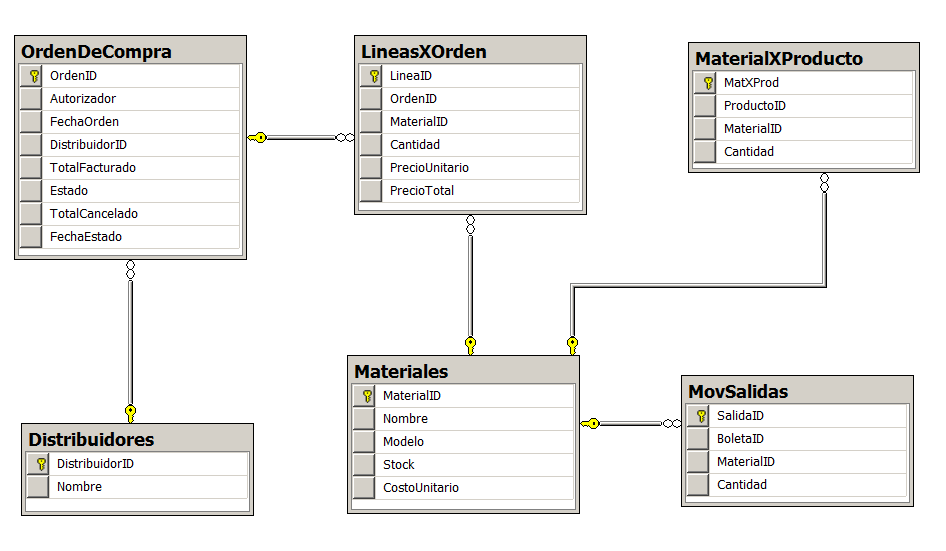
\includegraphics[width=1\textwidth]{diagInv.PNG}
\end{figure}

\begin{figure}[!ht]
  \caption{Diagrama de la base de datos de Ventas}
  \centering
    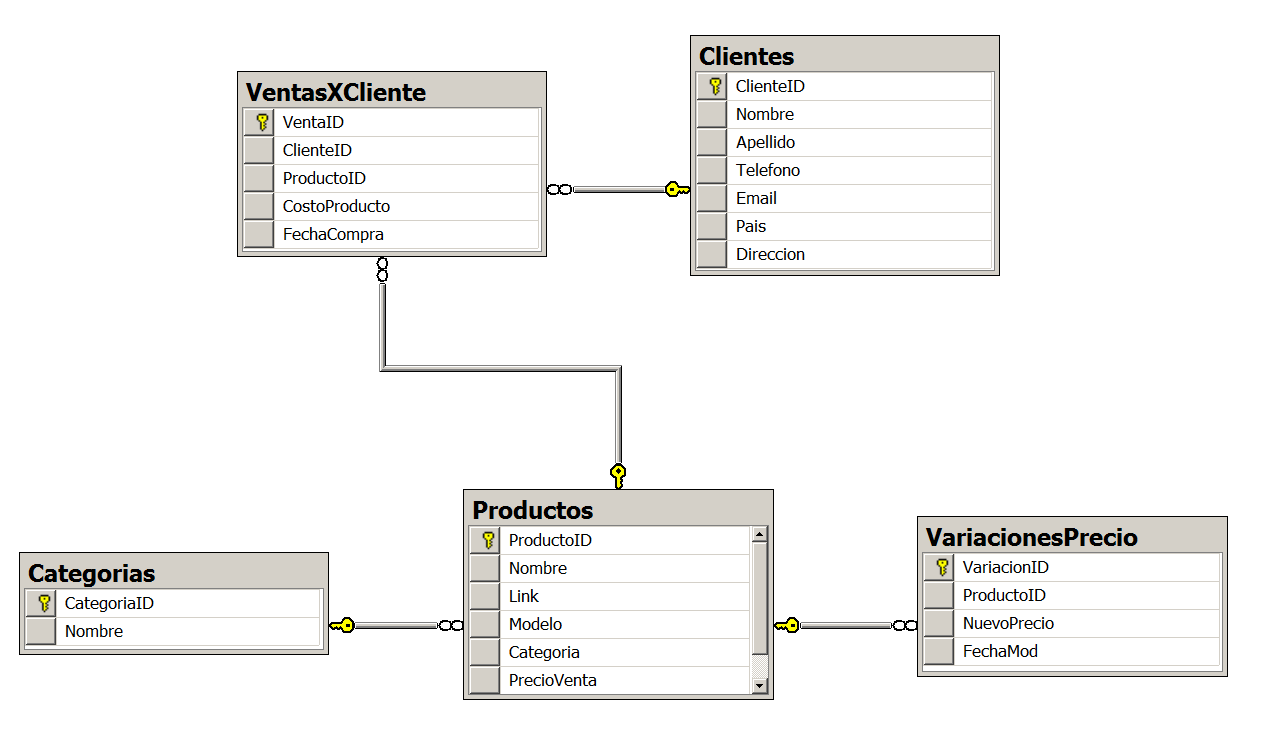
\includegraphics[width=1\textwidth]{diagVentas.PNG}
\end{figure}

\begin{figure}[!ht]
  \caption{Configuraci\'on de conexi\'on a Pentaho}
  \centering
    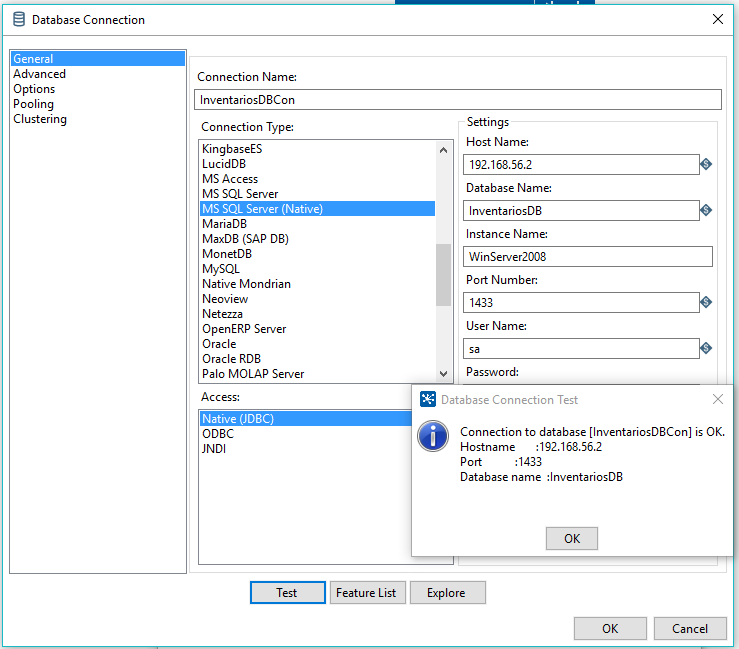
\includegraphics[width=1\textwidth]{pentahoDBCon1.PNG}
\end{figure}

\begin{figure}[!ht]
  \caption{Estados de las bases de datos replicadas}
  \centering
    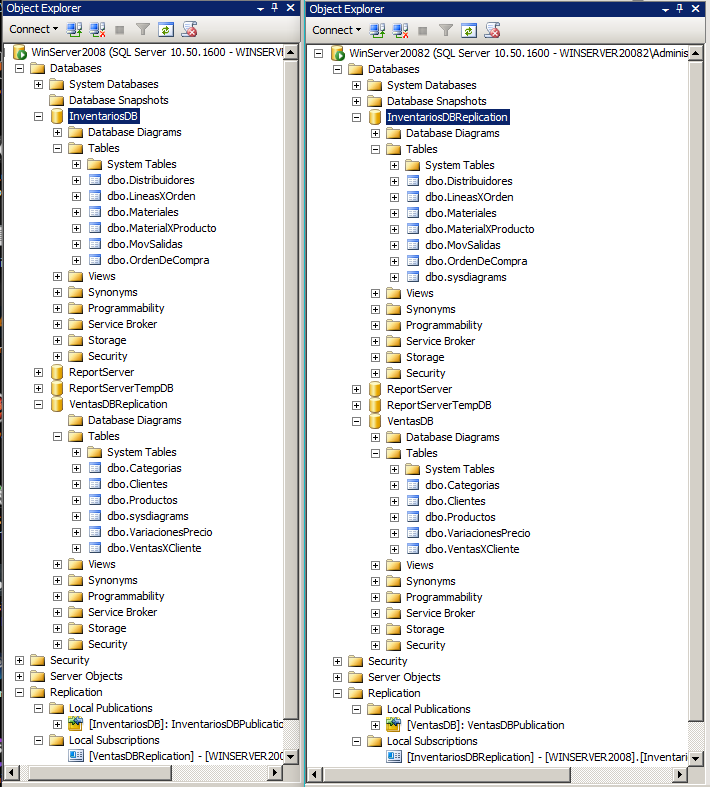
\includegraphics[width=1\textwidth]{replicacionFull.PNG}
\end{figure}

\begin{figure}[!ht]
  \caption{Reporte de Analisis de Despachos con dimensiones de Carriers y Pa\'is}
  \centering
    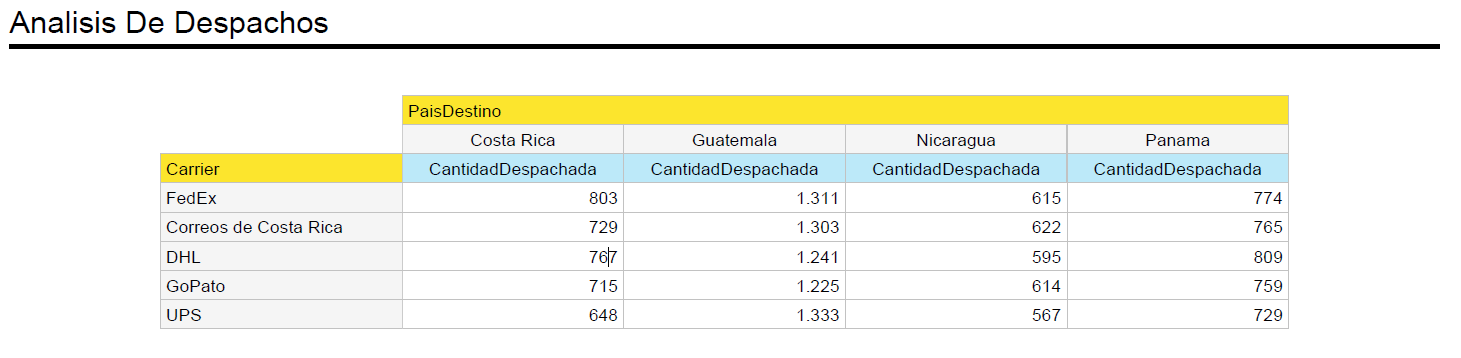
\includegraphics[width=1\textwidth]{analisis.PNG}
\end{figure}

\end{document}